\documentclass{standalone}
\usepackage{tikz}

\usetikzlibrary{calc}


\begin{document}

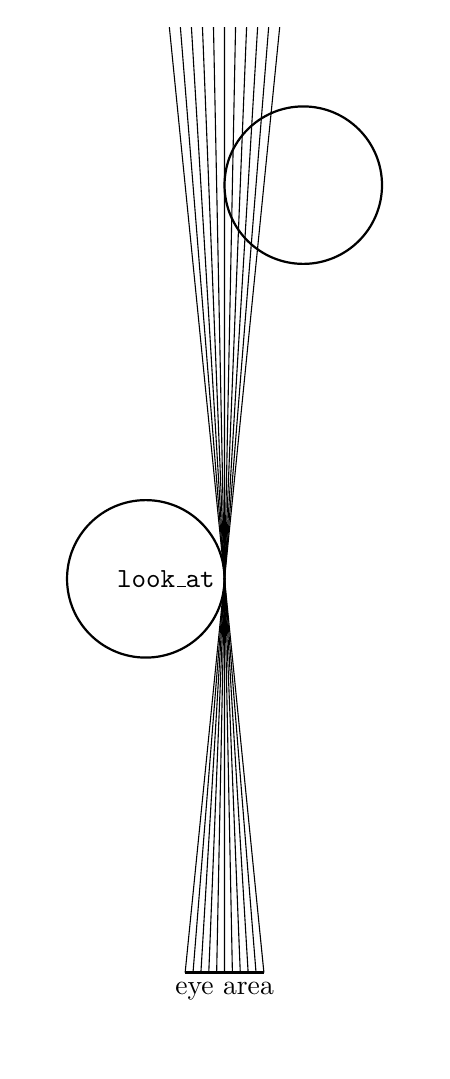
\begin{tikzpicture}
  \path[clip] (-2.5,-6) rectangle (2.5,7);
  \draw[thick] (-1,0) circle [radius=1cm];
  \draw[thick] (1,5) circle [radius=1cm];

  \draw[thick] (-0.5,-5) -- (0.5,-5) node[below,midway] {eye area};

  \coordinate (lookat) (0,5);

  \foreach \x in {-0.5,-0.4,...,0.51} {
    \draw[thin] (\x,-5) -- ($ (\x,-5) ! 5 ! (lookat) $);
  }

  \draw (lookat) circle [radius=0.01cm] node[left] {\tt look\_at};
\end{tikzpicture}

\end{document}